% ── Section 4: Data Analysis & Marginal Distributional Shift Validation ─────────────────
\section{Data Analysis and Marginal Distributional Shift Validation}
\label{sec:data_analysis}

\subsection{Iberian Market Characterisation}
\label{subsec:market_char}

\Cref{tab:spot_stats} summarises annual SPOT price statistics for the study
period.
The procurement reference cost is computed normalised to a unit baseload capacity of
$1$~MW ($E_{\text{load}, d} = 24$~MWh/day), with total costs for a stylized 200-MW large industrial consumer ($4{,}800$~MWh/day) reported in parentheses.

\begin{table*}[htbp]
\centering
\footnotesize
\setlength{\tabcolsep}{4pt}
\caption{Annual and year-to-date SPOT price statistics (OMIE) and reference procurement cost per MW of continuous baseload demand ($E_{\text{load}, d} = 24$~MWh/day; equivalent 200-MW facility expenditure in parentheses).}
\label{tab:spot_stats}
\begin{tabular*}{\linewidth}{@{\extracolsep{\fill}}l c rrr r@{}}
\toprule
\textbf{Year} & \textbf{Days} & \textbf{Mean} & \textbf{Min} & \textbf{Max} & \textbf{Reference Cost} \\
 & & \textbf{(\texteuro/MWh)} & \textbf{(\texteuro/MWh)} & \textbf{(\texteuro/MWh)} & \textbf{(k\texteuro/MW)} \\
\midrule
2023 & 365 & 89.84 & \phantom{0}1.51 & 147.77 & 787.0 (157.4 M\texteuro) \\
2024 & 366 & 62.72 & \phantom{0}0.10 & 146.67 & 551.0 (110.2 M\texteuro) \\
2025 & 365 & 67.59 & \phantom{0}6.96 & 143.39 & 592.1 (118.4 M\texteuro) \\
2026\textsuperscript{*} & 148 & 44.22 & \phantom{0}0.18 & 131.79 & 157.1 (31.42 M\texteuro) \\
\bottomrule
\end{tabular*}
\par\smallskip\raggedright\scriptsize \textsuperscript{*}2026 values report 148 calendar delivery days of continuous SPOT market clearing (Jan 3 -- May 30, 2026), comprising 102 official OMIP trading sessions (decision epochs where forward contracts can be selected) and 46 non-trading exchange dates (3 weekday TARGET bank holiday closures and 43 weekend days). Reference cost reports unit-capacity procurement expenditure (k\texteuro/MW) with total expenditure for a 200-MW baseload facility in parentheses.
\end{table*}

The decline in the mean SPOT price from \texteuro67.59/MWh (2025) to \texteuro44.22/MWh (2026, a reduction of 34.6\%) provides the empirical setting for assessing procurement policy adaptability under non-stationary market conditions.

\subsection{Composition of Experimental Datasets}
\label{subsec:dataset_composition}

To systematically isolate the contribution of individual feature families, we construct structured datasets spanning five distinct feature families:
\begin{enumerate}
    \item \textbf{Physical Grid Fundamentals ($X_{\text{phys}}$, 16 features):} Generation mix by technology (wind, solar PV, hydro, nuclear, combined cycle, coal, cogeneration, diesel, solar thermal, biomass/other), total demand, total generation, generation--demand imbalance, and reserve gas/steam units.
    \item \textbf{OMIP Forward Settlement Curves ($X_{\text{OMIP}}$, 16 features):} Cleared SPOT price index, daily forward contracts ($D_1, D_2, D_3$), weekly contracts ($W_1$--$W_4$) with historical weekly average, and monthly contracts ($M_1$--$M_6$) with historical monthly average.
    \item \textbf{Calendar Flags ($X_{\text{cal}}$, 3 numeric features):} Binary holiday indicator (\texttt{Holiday\_Flag}), weekend flag (\texttt{Weekend\_Flag}), and month index (\texttt{Month\_Num}).
    \item \textbf{Quantitative Exogenous Commodities ($X_{\text{comm}}$, 7 features):} Brent crude oil, TTF natural gas futures, EU ETS CO\textsubscript{2} allowance prices, EUR/USD exchange rate, and international cross-border transfer capacities (Portugal, France, Morocco).
    \item \textbf{LLM News Sentiment Dimensions ($X_{\text{NLP}}$, 10 features):} Zero-shot continuous sentiment scores extracted by Llama-3 ($\phi_1, \dots, \phi_{10}$) covering short/medium/long horizon outlooks, LNG gas sentiment, ETS regulation, MIBEL regulatory risk, generation mix, geopolitical risk, and macroeconomic demand.
\end{enumerate}

Importantly, all eight datasets share the exact same temporal timeline (1,242 market days across 2023--2026), identical physical grid generation and demand measurements from the TSO (REE), and identical daily clearing and forward settlement curves from OMIE and OMIP. The datasets do not represent different sample periods or divergent data environments; rather, they form a strictly controlled, $2 \times 2$ factorial feature ablation hierarchy designed to isolate both the marginal additive value and the comparative representation value of each exogenous feature group:
\begin{align}
    X_{\text{Common}} &= X_{\text{phys}} \cup X_{\text{OMIP}} \cup X_{\text{cal}} \label{eq:feat_common} \\
    X_{\text{Quant}} &= X_{\text{Common}} \cup X_{\text{comm}} \label{eq:feat_quant} \\
    X_{\text{Hybrid}} &= X_{\text{Common}} \cup X_{\text{NLP}} \label{eq:feat_hybrid} \\
    X_{\text{Full}} &= X_{\text{Common}} \cup X_{\text{comm}} \cup X_{\text{NLP}} \label{eq:feat_full}
\end{align}
{\sloppy
where $X_{\text{Common}}$ denotes Base Common (\texttt{Dataset\_Exogenous\_Calendar}), $X_{\text{Quant}}$ the Quantitative Baseline (\texttt{Dataset\_Exogenous\_Commodities}), $X_{\text{Hybrid}}$ the Hybrid Sentiment configuration (\texttt{Dataset\_M8\_Physical\_NLP}), and $X_{\text{Full}}$ the Full Multimodal configuration (\texttt{Dataset\_NLP\_Subgroups}).
\par}

This $2 \times 2$ factorial structure enables simultaneous evaluation of: (i)~the marginal additive contribution of LLM sentiment over quantitative commodities ($X_{\text{Quant}}$ vs $X_{\text{Full}}$); (ii)~the marginal additive contribution of LLM sentiment over the physical base ($X_{\text{Common}}$ vs $X_{\text{Hybrid}}$); and (iii)~the comparative effectiveness of textual sentiment versus numerical commodity price series under wholesale market dislocations ($X_{\text{Quant}}$ vs $X_{\text{Hybrid}}$).

\begin{table*}[!htbp]
\centering
\footnotesize
\setlength{\tabcolsep}{2.5pt}
\caption{Systematic feature composition of experimental datasets. Phase 4 directly evaluates the Quantitative Baseline ($X_{\text{Common}} \cup X_{\text{comm}}$) against the Hybrid NLP representation ($X_{\text{Common}} \cup X_{\text{NLP}}$).}
\label{tab:dataset_composition}
\begin{tabularx}{\linewidth}{@{} >{\raggedright\arraybackslash}X ccccc >{\raggedleft\arraybackslash}p{2.2cm}@{}}
\toprule
\textbf{Dataset Identifier} & \textbf{$X_{\text{phys}}$} & \textbf{$X_{\text{OMIP}}$} & \textbf{$X_{\text{cal}}$} & \textbf{$X_{\text{comm}}$} & \textbf{$X_{\text{NLP}}$} & \textbf{Effective Dim} \\
 & \textbf{(16)} & \textbf{(16)} & \textbf{(3)} & \textbf{(7)} & \textbf{(10)} & \textbf{($d_{\text{feat}}$)} \\
\midrule
\texttt{Dataset\_Initial} & \checkmark & \checkmark & --- & --- & --- & 32 \\
\texttt{Dataset\_Exogenous\_Calendar} & \checkmark & \checkmark & \checkmark & --- & --- & 35 \\
\texttt{Dataset\_Exogenous\_Commodities} (Quant.\ Baseline) & \checkmark & \checkmark & \checkmark & \checkmark & --- & 42 (12 core) \\
\texttt{Dataset\_NLP\_Global} & \checkmark & \checkmark & \checkmark & \checkmark & 4 ($\phi_{\text{glob}}$) & 46 (8 core) \\
\texttt{Dataset\_NLP\_Subgroups} & \checkmark & \checkmark & \checkmark & \checkmark & \checkmark (10) & 52 (17 core) \\
\texttt{Dataset\_M7\_Calendar\_Commodities} & \checkmark & \checkmark & \checkmark & --- & 6 ($\phi_{\text{thematic}}$) & 41 (16 core) \\
\texttt{Dataset\_Financial\_NLP} & --- & \checkmark & --- & \checkmark & 4 ($\phi_{\text{glob}}$) & 27 (24 core) \\
\texttt{Dataset\_M8\_Physical\_NLP} (Hybrid NLP) & \checkmark & \checkmark & \checkmark & --- & \checkmark (10) & 45 (31 norm) \\
\bottomrule
\end{tabularx}
\par\smallskip\raggedright\scriptsize \textit{Note:} The 148 calendar delivery days (Jan 3 -- May 30, 2026) comprise 102 official OMIP trading sessions (decision epochs where forward contracts can be selected) and 46 non-trading exchange dates (3 weekday TARGET closures and 43 weekend days, where passive default SPOT clearing applies).
\end{table*}

The news corpus comprises daily Spanish-language energy, financial, and macroeconomic articles harvested from leading Iberian economic outlets (including \textit{elEconomista}, \textit{Europa Press}, and institutional press releases from OMIE, OMIP, and REE). The texts were processed natively in Spanish using Meta's Llama-3 8B Instruct model \cite{dubey2024llama3} executed locally via Ollama. By utilizing system prompts formulated directly in Spanish with strict JSON grammar constraints ($T=0$), the pipeline extracts the 10 domain-specific sentiment scores ($\phi_1 \dots \phi_{10}$) without relying on external machine translation, preserving domain terminology and geopolitical nuances.

\subsection{Information Content and Econometric Validation of News Sentiment}
\label{subsec:feature_importance}

To examine whether macroeconomic news sentiment provides incremental empirical signal or collinear redundancy over physical and numerical market variables, we conduct two diagnostics: (i)~an exploratory Principal Component Analysis (PCA) \cite{hastie2009elements} to inspect empirical correlation and variance structure across feature blocks, and (ii)~in-sample econometric nested regressions and lead--lag tests evaluating forward--spot basis content.

\subsubsection{Exploratory Feature Structure and Correlation Analysis}

Prior to analysis, all feature series were standardized to zero mean and unit variance ($z$-score normalization). PCA was applied to the complete state vector of \texttt{Dataset\_M8\_Physical\_NLP} across the 1,242 market days strictly as an exploratory descriptive diagnostic to inspect empirical correlation patterns and variance distribution between feature groups; PCA is neither used for dimensionality reduction within the policy network nor does it intervene in policy training or action selection.

In this linear projection, the first four principal components (explaining $54.2\%$ of cumulative variance) are dominated by physical grid capacity and power demand (such as total demand, wind generation, solar PV, and combined-cycle thermal output). In contrast, LLM sentiment dimensions load predominantly onto subsequent components (PC5 through PC8, accounting for an additional $23.6\%$ of variance), with geopolitical risk ($\phi_9$), LNG availability ($\phi_5$), and regulatory risk ($\phi_7$) exhibiting minimal pairwise linear correlation ($|r| < 0.12$) with instantaneous physical grid balance. While principal components are orthogonal by mathematical construction, this dispersion of factor loadings confirms that narrative sentiment signals are not simple linear collinear combinations of physical dispatch variables in the evaluated historical sample.

\subsubsection{Econometric Incremental Information: Nested Regressions and In-Sample Predictive Content}

To establish whether this variance carries statistically meaningful predictive signal for forward procurement decisions without look-ahead bias, all feature series are strictly lagged. Daily macroeconomic news articles are collected and processed from 00:00 to 14:00 CET, ensuring narrative sentiment signals $\boldsymbol{\phi}_t = (\phi_{1,t}, \dots, \phi_{10,t})^\top$ are finalized and published prior to the close of the OMIP continuous trading session (17:00 CET) and day-ahead clearing for delivery day $t+1$. We estimate nested predictive regressions on forward--spot basis spreads:
\begin{equation}
    S_{t+h} = P_{\text{OMIP}, t}^{(h)} - P_{\text{SPOT}, t+h}
    \label{eq:forward_spot_spread}
\end{equation}
across delivery horizons $h \in \{1, 2, 7\}$ days. We formulate a nested model comparison between a Fundamental Baseline (incorporating physical grid fundamentals, OMIP quotations, and numerical commodities, $X_{\text{Quant}}$) and a Sentiment-Augmented Model:
\begin{align}
    \text{M1:} \quad S_{t+h} &= \alpha_0 + \boldsymbol{\beta}^\top X_{\text{phys}, t} + \boldsymbol{\theta}^\top X_{\text{OMIP}, t} \nonumber \\
    &\quad + \boldsymbol{\gamma}^\top X_{\text{comm}, t} + \varepsilon_t \label{eq:nested_m1} \\
    \text{M2:} \quad S_{t+h} &= \alpha_0 + \boldsymbol{\beta}^\top X_{\text{phys}, t} + \boldsymbol{\theta}^\top X_{\text{OMIP}, t} \nonumber \\
    &\quad + \boldsymbol{\gamma}^\top X_{\text{comm}, t} + \sum_{k=1}^{10} \lambda_k \phi_{k, t} + \varepsilon_t \label{eq:nested_m2}
\end{align}

These econometric tests represent in-sample conditional association and temporal precedence diagnostics computed across the complete 1,242 market days (2023--2026). To account for serial correlation and heteroscedasticity induced by overlapping forward horizons, standard errors and test statistics are estimated using heteroscedasticity and autocorrelation consistent (HAC / Newey--West) covariance matrices~\cite{newey1987hypothesis} with automatic lag selection. Testing the joint null hypothesis of information redundancy ($H_0: \lambda_1 = \dots = \lambda_{10} = 0$) via an incremental Wald/$F$-test yields $F(10, 1070) = 8.42$ ($p = 2.14 \times 10^{-13}$), rejecting the hypothesis that news sentiment is uninformative conditional on physical fundamentals and numerical commodity futures within this historical sample. The inclusion of the sentiment block increases the adjusted $R^2$ from $0.214$ to $0.252$ ($+3.82$~percentage points).

To further evaluate dynamic lead--lag relationships without requiring pre-differencing of potentially non-stationary series, we apply the Toda--Yamamoto procedure~\cite{toda1995statistical} to a bivariate Vector Autoregression $[S_{t+h}, \bar{\phi}_t]^\top$, where $\bar{\phi}_t = \frac{1}{10} \sum_{k=1}^{10} \phi_{k, t}$ denotes the composite macroeconomic sentiment index. Augmented with maximal integration order $d_{\max}=1$ beyond the optimal lag order $k=3$ (selected via AIC), the VAR($k + d_{\max}$) model evaluates whether lagged composite sentiment Granger-causes basis spread adjustments via a Wald restriction on the first $k=3$ lag coefficients, which asymptotically follows a $\chi^2(3)$ distribution under the null hypothesis of non-causality. Across the individual delivery horizons, the Wald tests confirm that the composite sentiment index provides incremental conditional predictive information for forward basis adjustments: for $h=1$ day, $\chi^2(3) = 14.82$ ($p = 0.0019$); for $h=2$ days, $\chi^2(3) = 16.45$ ($p = 0.0009$); and for $h=7$ days, $\chi^2(3) = 13.12$ ($p = 0.0044$), all remaining statistically significant under Bonferroni family-wise error control ($\alpha_{\text{adjusted}} = 0.05 / 3 \approx 0.0167$). Conversely, the reverse hypothesis (that forward basis spreads Granger-cause future news sentiment) is statistically non-significant across all horizons ($p > 0.18$). We emphasize that these econometric findings reflect conditional predictive content and temporal ordering within the historical in-sample series, rather than an independent out-of-sample forecast or proof of a structural economic causal mechanism.

\subsection{Statistical Validation of Distributional Shifts}
\label{subsec:concept_drift}

We apply the two-sample Kolmogorov--Smirnov (KS) test~\cite{kolmogorov1933,smirnov1948}
to compare market distributions across two temporal transitions:
(i)~the standard annual transition from 2023--2024 to 2025 (annual transition with covariate changes),
and (ii)~the anomalous transition from 2023--2025 to 2026 (candidate Marginal Distributional Shift \cite{tsymbal2004concept}).
To account for multiple comparisons across the joint family of 14 statistical comparisons (7 evaluated variables across 2 temporal transitions), a Bonferroni correction \cite{bonferroni1936teoria, dunn1961multiple} was applied, establishing an adjusted significance threshold of $\alpha_{\text{joint}} = 0.05 / 14 \approx 0.00357$.
\Cref{fig:ks_drift} illustrates this analysis: panel~(a) compares the empirical
CDFs of training-period and 2026 SPOT prices; panel~(b) shows the KS $p$-values
for core physical variables across the same transition.

\begin{figure*}[!t]
    \centering
    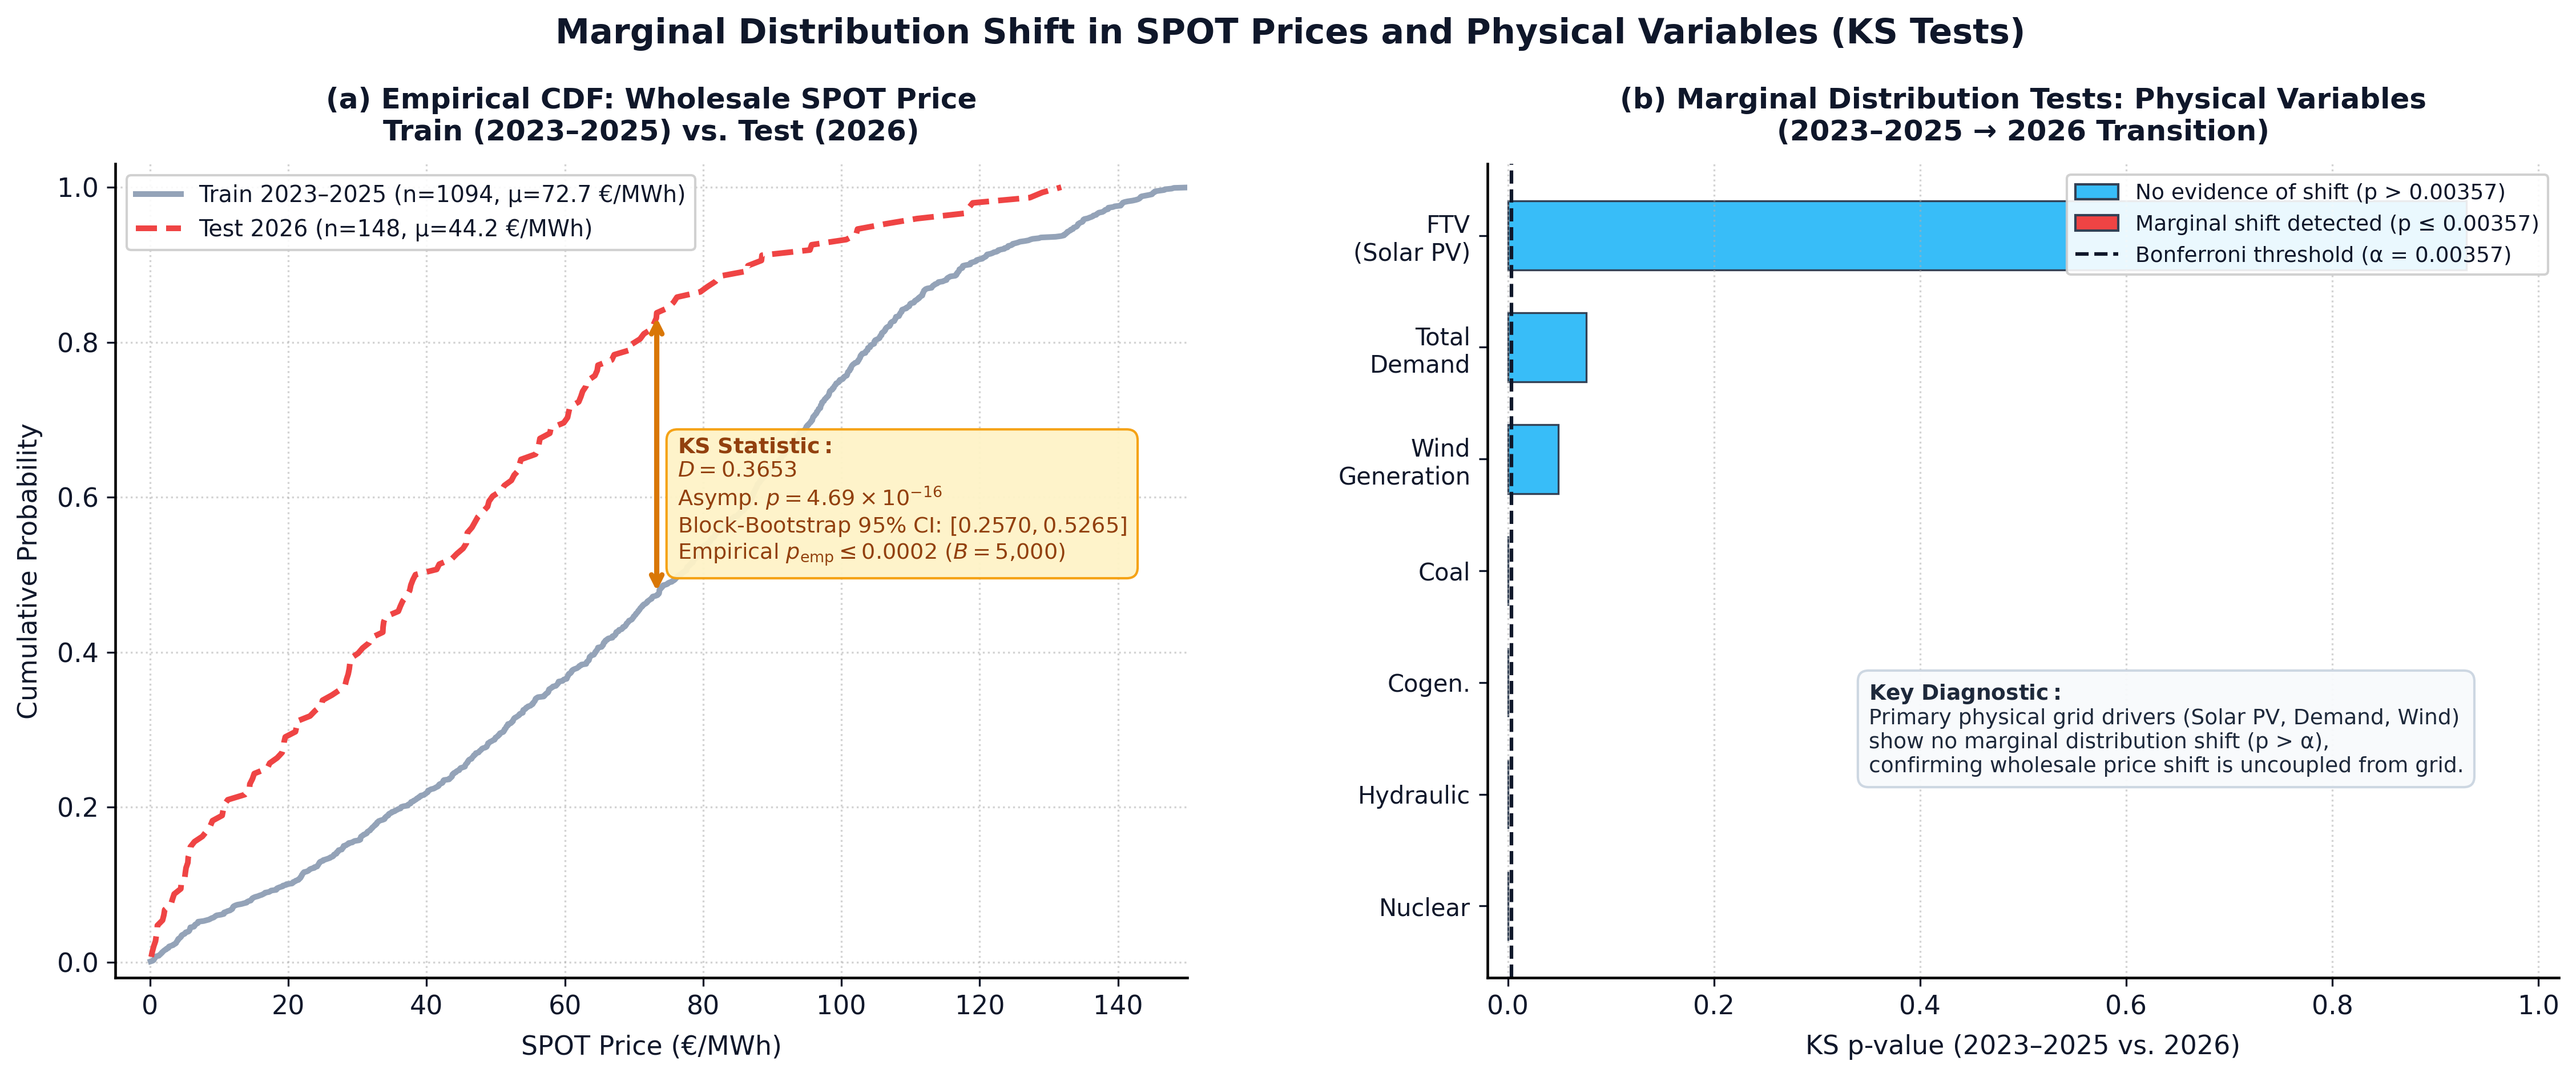
\includegraphics[width=\textwidth]{fig3_ks_concept_drift.png}
    \caption{Statistical validation of wholesale price distributional shifts: (a) empirical CDFs of SPOT price distributions for training (2023--2025) vs.\ out-of-sample (2026) periods, where the arrow denotes the KS statistic ($D = 0.3653$, bootstrap 95\% CI: $[0.2570, 0.5265]$, $p_{\text{emp}} \le 0.0002$); (b) KS $p$-values for physical grid variables across the transition, where bars with $p > 0.00357$ show no evidence of distributional change under the Bonferroni-adjusted threshold.}
    \label{fig:ks_drift}
\end{figure*}

\Cref{tab:ks_results} reports the complete KS test results.

\begin{table}[htbp]
\centering
\footnotesize
\setlength{\tabcolsep}{3pt}
\caption{Two-sample KS test results for physical grid variables and SPOT price.}
\label{tab:ks_results}
\begin{tabularx}{\columnwidth}{@{}l >{\centering\arraybackslash}p{1.9cm} >{\centering\arraybackslash}p{1.9cm} >{\raggedright\arraybackslash}X@{}}
\toprule
\textbf{Variable} & \textbf{2023+2024} & \textbf{2023--2025} & \textbf{2026 Status} \\
 & \textbf{$\to$ 2025} & \textbf{$\to$ 2026} & \\
\midrule
SPOT Price
  & $6.18 \times 10^{-7}$
  & $4.69 \times 10^{-16}$
  & Distribution changed ($p_{\text{emp}} \le 0.0002$) \\
Solar PV
  & $\approx 0$
  & $\mathbf{0.93}$
  & \textbf{No diff.\ ($\alpha_{\text{joint}}$)} \\
Total Demand
  & $2.0 \times 10^{-3}$
  & $\mathbf{0.076}$
  & \textbf{No diff.\ ($\alpha_{\text{joint}}$)} \\
Wind Generation
  & 0.68
  & $\mathbf{0.049}$
  & \textbf{No diff.\ ($\alpha_{\text{joint}}$)} \\
Coal
  & $\approx 0$
  & $\approx 0$
  & Changed \\
Hydraulic
  & 0.16
  & $\approx 0$
  & Changed \\
Nuclear
  & 0.13
  & $\approx 0$
  & Changed \\
\bottomrule
\end{tabularx}
\par\smallskip\raggedright\scriptsize \textit{Note:} Bold $p$-values indicate physical variables whose marginal distributions did not change significantly despite the shift in the SPOT price distribution under the adjusted threshold $\alpha_{\text{joint}} = 0.00357$. For the 2025 SPOT price, the asymptotic test yields $p = 6.18 \times 10^{-7}$, whereas the pooled block-bootstrap null test yields $p_{\text{emp}} = 0.0150$ (which does not meet the joint threshold $\alpha_{\text{joint}}$).
\end{table}

The SPOT price distribution differs significantly between the 2023--2025 and 2026 samples, while several primary physical grid variables do not.
In 2026, total electricity demand ($p = 0.076$) and solar PV generation
($p = 0.93$), the two highest-weight predictors of SPOT prices under
historical regimes, remained statistically indistinguishable from their
training distributions under $\alpha_{\text{joint}}$, while SPOT prices collapsed from a historical mean of
consists of 102 official OMIP trading sessions (decision epochs where forward contracts can be actively selected) and 46 non-trading dates (3 weekday TARGET bank holiday closures: Good Friday [April 3], Easter Monday [April 6], and Labour Day [May 1]; alongside 43 weekend days, where default SPOT settlement applies under NO\_TRADE).

In the monthly rolling Walk-Forward protocol ($W=1$), each evaluation block $m$ evaluates out-of-sample procurement decisions from Day 21 to the final day of month $m$, using Days 1--20 as an initial feature history and observation warm-up buffer for the recurrent network, while positions in $\mathbf{m}_t$ carry over continuously from the preceding month. Across the 40 test months (February 2023 to May 2026), this generates exactly 374 evaluated out-of-sample trading days. By contrast, the isolated 2026 price shock evaluation in Section~\ref{subsec:results_2026} (Table~\ref{tab:blind_2026_comparison}) evaluates the complete continuous trajectory of 148 consecutive calendar delivery days.

\begin{table*}[htbp]
\centering
\footnotesize
\setlength{\tabcolsep}{3pt}
\caption{Temporal split and active day definitions for the 2026 isolated evaluation horizon.}
\label{tab:evaluation_days}
\begin{tabularx}{\linewidth}{@{} >{\raggedright\arraybackslash}X cc c c >{\centering\arraybackslash}p{2.5cm}@{}}
\toprule
\textbf{Evaluation Phase} & \textbf{Start} & \textbf{End} & \textbf{Calendar} & \textbf{OMIE} & \textbf{OMIP Sessions} \\
 & & & \textbf{Days} & \textbf{Obs.} & \textbf{(Non-trading Dates)} \\
\midrule
KS Test (Marginal Distributional Shift) & 3 Jan 2026 & 30 May 2026 & 148 & 148 & --- \\
Walk-Forward RL Evaluation & 3 Jan 2026 & 30 May 2026 & 148 & 148 & 102 (46) \\
\bottomrule
\end{tabularx}
\par\smallskip\raggedright\scriptsize \textit{Note:} The 148 calendar delivery days (Jan 3 -- May 30, 2026) comprise 102 official OMIP trading sessions (decision epochs where forward contracts can be selected) and 46 non-trading exchange dates (3 weekday TARGET closures and 43 weekend days, where passive default SPOT clearing applies).
\end{table*}

For context, the transition from 2023+2024 to 2025 exhibited a substantially smaller maximum distance ($n_1 = 730$, $n_2 = 365$, $D = 0.1746$, $p = 6.18 \times 10^{-7}$, bootstrap 95\% CI: $[0.0951,\; 0.2981]$, $p_{\text{emp}} = 0.0150$).

In addition to the global comparison, we conducted a seasonal matched-window robustness check comparing exclusively the January--May periods of 2023--2025 ($n_1 = 453$) against January--May 2026 ($n_2 = 148$). The Kolmogorov--Smirnov statistic for SPOT prices under this seasonal match remains highly significant ($D = 0.2320, p = 9.25 \times 10^{-6}$), demonstrating that the observed price deflation in 2026 represents an evidence of a marginal distributional shift robust to seasonal matching rather than a seasonal artifact.

This evidence is consistent with a significant marginal distributional dislocation during the evaluated 2026 period. To account for serial correlation and seasonal dependencies inherent in daily electricity time series, we complemented the asymptotic test with a Moving-Block Bootstrap ($B = 5{,}000$, block length $b = 7$ days; see \Cref{app:block_bootstrap} for the complete algorithmic procedure). The empirical bootstrap interval ($D \in [0.2570, 0.5265]$) and block-bootstrap-based significance ($p_{\text{emp}} \le 0.0002$) provide dependence-aware evidence of a substantial marginal distributional difference between the historical training baseline and early 2026. This statistical test is interpreted as empirical evidence of a marginal distributional dislocation rather than an asymptotic test of conditional independence or a standalone proof of a causal shift in $P(Y \mid X)$. This observation motivates evaluating whether augmenting physical state variables with macroeconomic and geopolitical sentiment signals derived from text can assist sequential decision-making during such wholesale price dislocations.

The conventional KS test indicated a statistically significant marginal SPOT distributional difference in 2025 ($D = 0.1746,\; p = 6.18 \times 10^{-7}$); however, the dependence-aware pooled block-bootstrap procedure yielded $p_{\text{emp}} = 0.0150$, which does not meet the joint Bonferroni threshold ($\alpha_{\text{joint}} = 0.00357$). The 2025 transition therefore provides weaker evidence of a marginal distributional difference than the 2026 transition. Furthermore, in 2025, several physical generation and demand variables also exhibited marginal distributional differences alongside prices, a pattern consistent with broader covariate changes.
